\section{Model Construction and Implementation}Translate the following LaTeX content:\subsection{Career Choice as a Modeling Decision}Translate the following LaTeX content:The premise of the problem requires selecting one profession each from the STEM, skilled trades, and arts fields.  
We do not treat this step as an ad hoc assumption (subjective choice), but explicitly model the profession selection as an optimization problem.  
This ensures that the subsequent analysis of AI-driven impacts and educational recommendations is built upon a reproducible and data-driven framework.  
The core objective of profession selection is not representativeness of all professions, but \emph{explanatory contrast}.  
Specifically, the task structures of the three professions should exhibit significant differences in how they interact with GenAI.  
In addition to mechanistic contrast, the problem explicitly emphasizes data-driven reasoning and subsequent policy recommendations. Therefore, the selected professions must also have comprehensive data support and policy relevance.\subsubsection{Objective Parameterization of Occupational Characteristics Based on O*NET}Translate the following LaTeX content:To avoid subjective assignment of the occupational characteristic parameters $\textit{digit}(x)$, $\textit{physical}(x)$, and $\textit{iprisk}(x)$, we adopt the \textbf{O*NET} occupational database maintained by the U.S. Department of Labor as a unified data source. Detailed information on the data sources is summarized in Section 3.
Based on expert surveys and practitioner feedback, O*NET provides a large number of \emph{numerical scale descriptors} for each occupation. Most indicators are naturally given as real numbers between $0$ and $100$, making them suitable for direct use in quantitative modeling.We do not attempt to find a "single correct" metric for each dimension. For each feature axis, we select a small number of semantically directly corresponding and downloadable O*NET descriptors and use them as proxy variables for that axis.Based on the problem statement and data availability constraints, we identify three dominant dimensions that govern the heterogeneity of AI impacts across occupations:
\begin{itemize}
    \item \textbf{Digitalization degree $digit(x)$}: The extent to which core tasks can be represented, automated, or enhanced digitally;
    \item \textbf{Physical anchoring $physical(x)$}: The degree of reliance on on-site physical presence or manual interaction with the environment for task execution;
    \item \textbf{Intellectual property and attribution risk $iprisk(x)$}: The sensitivity of value creation to authorship, originality, and ownership.
\end{itemize}Each candidate occupation $x$ is represented by a normalized three-dimensional feature vector
\begin{equation}
    f(x)=\big(digit(x),\,physical(x),\,iprisk(x)\big)\in[0,1]^3,
\end{equation}
where higher values indicate a stronger presence of the corresponding feature.For three occupational categories $(x_1,x_2,x_3)$ sampled from STEM, skilled trades, and arts respectively, we define the contrast between two occupations as the Euclidean distance between their feature vectors:
\begin{equation}
    \Delta(x_i,x_j)=\lVert f(x_i)-f(x_j)\rVert_2.
\end{equation}Define the data availability score \(D(x_k)\), which reflects the ease and richness of obtaining data related to that occupation. The overall selection objective is formulated as  
\begin{equation}  
    \max_{x_1\in STEM,\;x_2\in Trade,\;x_3\in Arts}  
    \left(  
    \sum_{i<j}\Delta(x_i,x_j)  
    +\lambda\sum_{k=1}^{3}D(x_k)  
    \right),  
\end{equation}  
where \(\lambda\) is a weighting coefficient that balances interpretability comparison with empirical feasibility.This formula does not claim global optimality across all possible careers.  
Instead, it generates a carefully constructed set of high-contrast careers that maximizes analytical clarity under realistic data and time constraints.\paragraph{Normalization and Reproducibility}For each occupation $x$, let $v_m(x)$ denote its raw score ($0$--$100$) under the O*NET descriptor $m$.
We apply min-max normalization across the entire set of occupations:
\begin{equation}
    z_m(x)=\frac{v_m(x)-\min_{y}v_m(y)}{\max_{y}v_m(y)-\min_{y}v_m(y)} \in [0,1],
\end{equation}
and take the equally weighted average of multiple descriptors under the same feature axis to obtain $\textit{digit}(x)$, $\textit{physical}(x)$, and $\textit{iprisk}(x)$.
This process is entirely based on publicly available data and explicit rules, ensuring the reproducibility and auditability of the parameter values.We visualized the three-dimensional heterogeneity and its two-dimensional projections to verify that the selected occupations occupy distinct regions in the feature space (Figure~\ref{fig:heterogeneity3d} and Figure~\ref{fig:heterogeneity2d}).\begin{figure}[H]
\centering
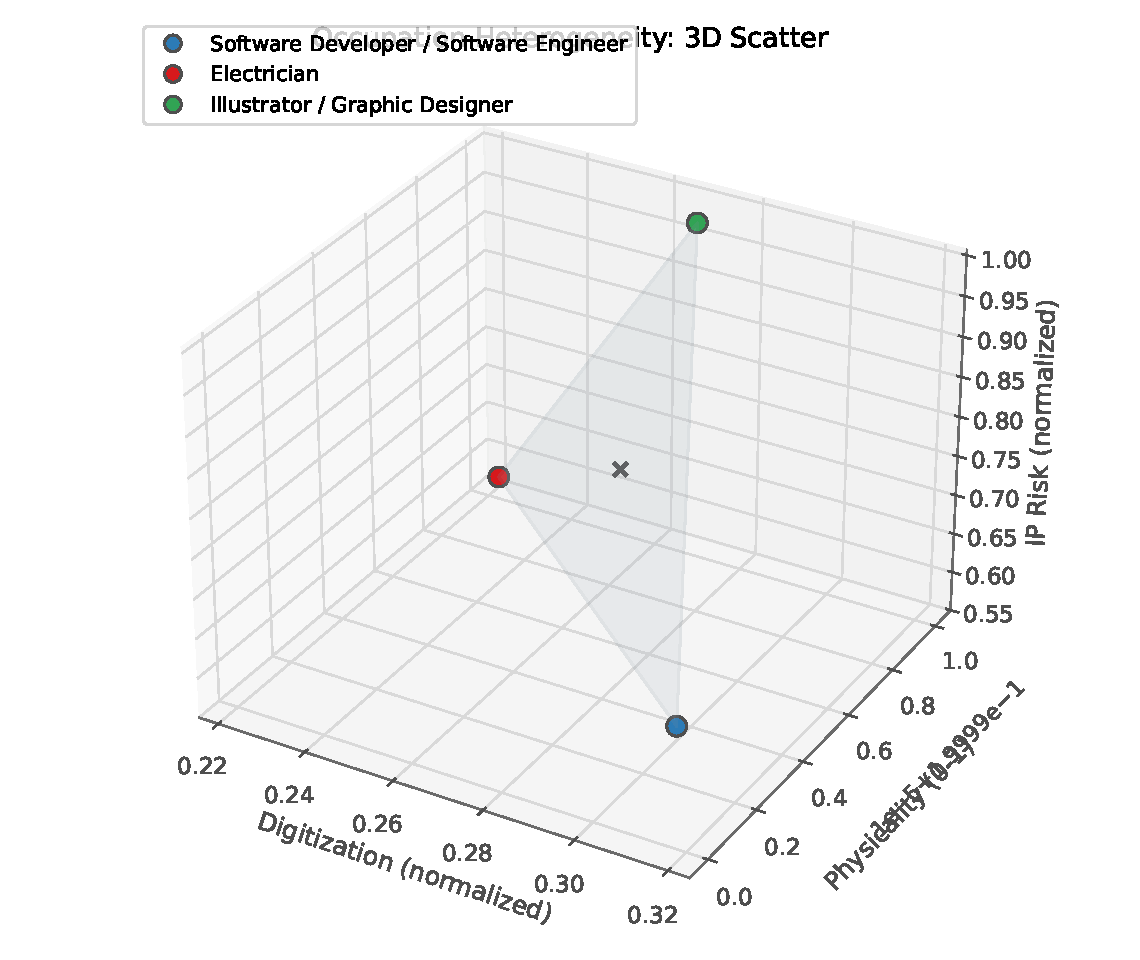
\includegraphics[width=0.78\textwidth]{figures/fig1_heterogeneity_3d.pdf}
\caption{Three-dimensional heterogeneity of selected STEM, skilled trade, and artistic occupations based on O*NET descriptors (globally normalized).}
\label{fig:heterogeneity3d}
\end{figure}\begin{figure}[H]
\centering
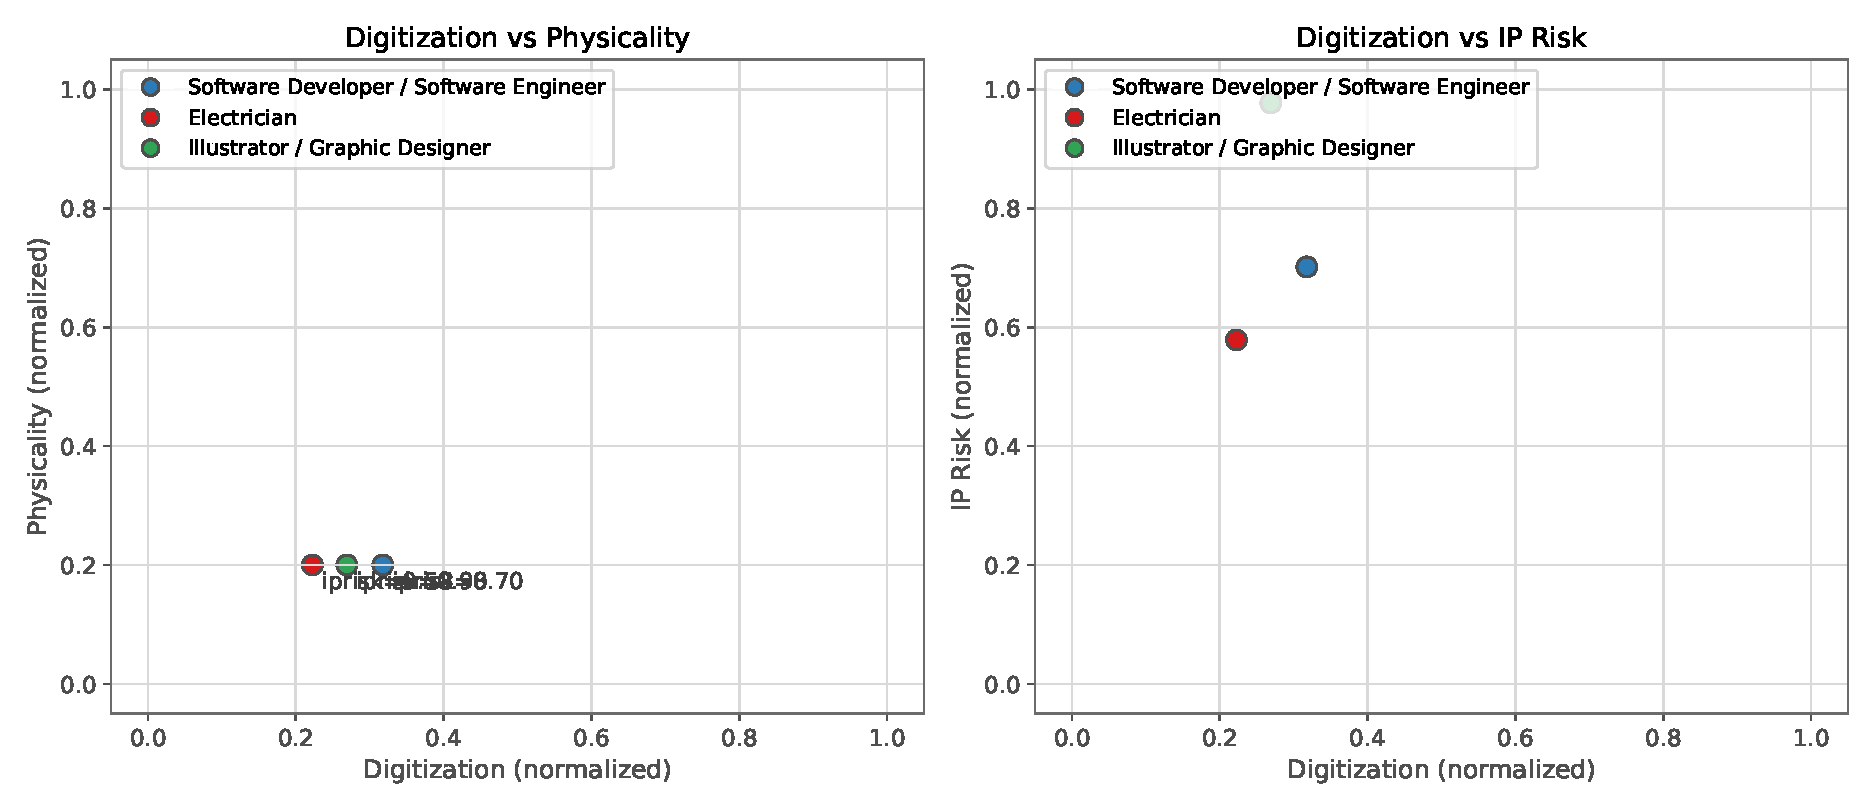
\includegraphics[width=0.92\textwidth]{figures/fig2_projections.pdf}
\caption{Two-dimensional projection of the heterogeneous space; annotations report the values of the remaining axes to enhance interpretability (global normalization).}
\label{fig:heterogeneity2d}
\end{figure}\subsubsection{Revision and Final Configuration of Selected Careers}Translate the following LaTeX content:In the initial scheme, we selected structural/civil engineers as the STEM profession. However, upon further examination of the distribution of the three professions along the dimensions of "task structure" and "physical constraints," we found that this choice exhibits some similarity with the trade profession (electricians) on the "physical anchoring strength" axis, which may weaken the contrast among the three professions in the mechanism space.To maximize the heterogeneity of the task structure and enhance the identifiability of subsequent GenAI impact mechanisms, we revise the STEM endpoint by replacing it with \textbf{software developers/software engineers}.This revision does not alter the structure of the original selection model; it only adjusts the positions of occupational endpoints in the feature space: software developers exhibit an extremely high degree of digitalization and an extremely low level of physical anchoring, thereby significantly increasing their distance from electricians in the feature vector $f(x)$ and enhancing the overall contrastive objective function value.It must be emphasized that we do not assume that the software development profession will be simply "replaced" by GenAI. Instead, this profession is more likely to undergo a \textbf{restructuring of task composition}: the proportion of coding and boilerplate implementation decreases, while the proportion of tasks such as requirement clarification, system architecture design, verification testing, and security and compliance responsibilities increases. It is precisely this shift from "execution-oriented tasks" to "verification and responsibility-oriented tasks" that makes software development an ideal STEM endpoint for studying the impact mechanisms of GenAI.After completing this revision, the final configurations of the three selected occupations are as follows:\begin{itemize}
    \item \textbf{STEM: Software Developer/Software Engineer.}
    High degree of digitalization, low physical anchoring; GenAI can directly intervene in core tasks, but primarily manifests as task redistribution rather than occupational obsolescence.

    \item \textbf{Skilled Trade: Electrician.}
    High physical anchoring, strong on-site constraints; AI mainly serves as a planning, diagnostic, and assistive tool, making it difficult to replace core operational tasks.

    \item \textbf{Arts: Commercial Illustrator/Graphic Designer.}
    High sensitivity regarding intellectual property and attribution; GenAI directly influences the form of output and the mechanisms of value pricing.
\end{itemize}\subsection{Model Selection for Career Evolution}Translate the following LaTeX content:The second core requirement of the problem is to construct a \emph{data-driven} model for the future evolution of professions.  
Before introducing formal equations, we first define the meaning of "future evolution" in a computable sense, and then systematically evaluate alternative modeling approaches, ensuring that the model selection itself does not become an implicit assumption.\subsubsection{Computable Definition of Future Evolution}Translate the following LaTeX content:We characterize the future evolution of occupation \(i\) through two primary outputs:
\begin{itemize}
    \item \textbf{Occupational Demand}: The temporal evolution of employment demand \(E_i(t)\) over a 10-year horizon under rapid, moderate, and slow GenAI adoption scenarios;
    \item \textbf{Task Structure}: The reallocation of task weights \(T_i(t)\) within the occupation, indicating which tasks expand, contract, or are restructured.
\end{itemize}This definition ensures that professional-level outcomes stem from task-level mechanisms, rather than being directly imposed.\subsubsection{Comparison of Candidate Modeling Methods}Translate the following LaTeX content:We consider three representative approaches for modeling career evolution:\paragraph{Method A: Task Aggregation Impact Model}This method treats occupations as weighted combinations of tasks.  
The substitution and enhancement effects driven by GenAI are specified at the task level and then aggregated to the occupational level using task weights.  
Most parameters can be constructed from O*NET task data \cite{onet2025database} and publicly available AI exposure scales \cite{freyosborne2017}, ensuring transparency and reproducibility.\paragraph{Method B: Time Series Model for Recruitment Information}This method infers occupational changes from trends in AI-related keywords and skill requirements in job postings.  
While closely tied to market signals, it faces identification challenges and high data processing overhead, making it unsuitable as the primary modeling framework.\paragraph{Method C: Agent-Based Simulation}Agent-based models simulate strategic interactions among firms, workers, and educational institutions.  
Although rich in narrative, they require extensive calibration and introduce substantial model complexity, which conflicts with transparency requirements under strict page limits.\subsubsection{Final Model Selection}Translate the following LaTeX content:Based on the above comparison, we adopt the Task Aggregation Impact Model (Method A) as the primary framework.  
The motivation for this selection is:  
\begin{itemize}  
    \item \textbf{Mechanism Clarity}: Occupational changes are explicitly derived from task-level effects;  
    \item \textbf{Data Alignment}: Key parameters are based on publicly available occupational data \cite{onet2025database,censuspseo2025};  
    \item \textbf{Controllable Complexity}: The model maintains interpretability, making it suitable for scenario and sensitivity analysis;  
    \item \textbf{Transferability}: The framework can be easily extended to other occupations or educational pathways \cite{ncescip2020soc2018}.  
\end{itemize}Method B is reserved for potential validation or supplementary analysis, while Method C is excluded from the primary analysis due to calibration and transparency issues.\subsection{Dynamic Model of Task Aggregation for Occupational Evolution}Translate the following LaTeX content:After justifying the task aggregation approach, we now present its mathematical formulation.
We adopt a task-to-occupation framework with minimal structure: GenAI adoption $A(t)$ enters as an exogenous driver, substitution and enhancement are specified at the task level, and the net occupational impact is aggregated via task weights, yielding the dynamic trajectory of occupational demand $E_i(t)$.\subsubsection{Task Aggregation and Occupational Dynamics}Translate the following LaTeX content:Let occupation \(i\) consist of tasks \(j=1,\dots,J_i\) with weights \(w_{ij}\) satisfying
\begin{equation}
    \sum_{j=1}^{J_i} w_{ij} = 1.
\end{equation}
For each task \(j\), let \(s_{ij}\in[0,1]\) denote the substitution intensity and \(c_{ij}\in[0,1]\) denote the enhancement (complementarity) intensity.
Define the occupation-level aggregate effects as
\begin{equation}
    \alpha_i=\sum_{j=1}^{J_i} w_{ij}\,s_{ij},\qquad
    \beta_i=\sum_{j=1}^{J_i} w_{ij}\,c_{ij}.
\end{equation}Let $E_i(t)$ be the employment demand for occupation $i$ at time $t$, and $g_i$ capture the baseline growth/decay from non-AI factors (estimated from public trends or set to $0$ under scenario analysis).  
Given a family of adoption trajectory scenarios $A(t) \in [0,1]$ (fast/medium/slow), we model occupational evolution as  
\begin{equation}
    \frac{dE_i(t)}{dt}=E_i(t)\Big(g_i + A(t)\,(\beta_i-\alpha_i)\Big).
\end{equation}
This formulation ensures that occupational outcomes stem from task-level mechanisms, supporting interpretability, reproducibility, and data-driven reasoning.\subsection{GenAI Capability Dimension Scoring from Authoritative Reports: Scale Definition and Evidence Narrative}Translate the following LaTeX content:To replace the subjective "keyword tagging" approach, we adopt capability scores derived from authoritative evaluations and official technical reports.  
These scores quantify GenAI's \textbf{substitution} and \textbf{enhancement} capabilities across key dimensions of software development tasks, providing an auditable basis for mapping software developer task DNA to $(s,c)$ inputs.\subsubsection{Scale Definition}Translate the following LaTeX content:We use three levels (low/medium/high) to represent GenAI capabilities, encoded as $0.25$, $0.50$, and $0.75$:
\begin{itemize}
    \item \textbf{Low (0.25)}: GenAI has limited autonomous capability in this task type and cannot reliably deliver satisfactory results without human intervention; it can only replace a small portion of the work but can still provide assistance under human supervision.
    \item \textbf{Medium (0.50)}: GenAI performs moderately, completing some tasks or providing useful suggestions, but still requires human review and collaboration; it cannot independently replace human execution.
    \item \textbf{High (0.75)}: GenAI performs strongly, approaching professional human levels in many subtasks; with appropriate constraints and validation, it can handle most of the workflow and provide significant enhancement, though it is still not perfect.
\end{itemize}\noindent\textbf{Note:} The values of $0.25/0.50/0.75$ are rough modeling encodings rather than precise measurements. All levels are based on publicly released reports and comparative experiments from the past two years.\subsubsection{Evidence of Capabilities by Task Type (Narrative Argument)}Translate the following LaTeX content:\paragraph{Code Generation}\textbf{Substitution: High (0.75); Enhancement: High (0.75).}
GenAI has demonstrated strong performance in automated code generation. OpenAI GPT-4 achieves $67.0\%$ pass@1 on HumanEval, significantly higher than GPT-3.5's $48.1\%$; Anthropic Claude 2 reaches $71.2\%$ on the same benchmark. This indicates that leading models can correctly solve over half of typical coding problems. Google CEO Sundar Pichai stated that approximately $25\%$ of Google's new code is generated by AI tools, reflecting a significant productivity boost: given an intent or comment, models can generate a large amount of draft code and accelerate development. For simple modules, models can partially substitute manual coding. However, outputs still require human review and testing to reduce logical errors and security issues. Overall, coding/implementation is one of the most substitutable and enhancing domains for GenAI.\paragraph{Testing and Verification}\textbf{Substitution: Medium (0.50); Enhancement: High (0.75).}
GenAI performs moderately in generating test cases and supporting verification, but is improving. Research reports indicate that LLM-generated unit tests can achieve coverage comparable to advanced automated tools and are often more readable. For example, experiments guided by static analysis at IBM Research found that GPT-based systems can generate competitive Java/Python unit tests in terms of coverage and defect detection capability, while producing developer-friendly tests. This supports strong enhancement in routine function-level verification. However, generated tests may target irrelevant scenarios or have weak assertions, requiring manual review; thus, full substitution remains difficult. In practice, GenAI can significantly reduce manual test writing and accelerate result checking, while humans verify test correctness.\paragraph{Debugging and Error Fixing}\textbf{Substitution: Low (0.25); Enhancement: Medium (0.50).}
End-to-end debugging remains a weakness: autonomous success rates are relatively low, but the auxiliary value is evident. A 2025 Microsoft Research study reported that even with debugger tool access, the best model (Anthropic Claude 3.7 Sonnet) solved only $48.4\%$ of 300 curated debugging tasks on average, while other models achieved around $30\%$. This indicates that GenAI cannot fully replace manual debugging. Limitations include ineffective use of debugging signals, poor strategy selection, and a lack of step-by-step reasoning traces. Therefore, substitution is rated low. Meanwhile, enhancement is evident: with logs or exception traces, models can propose useful fixes; in some setups, "self-debugging" via few-shot demonstrations improves success rates by approximately $2\%$--$12\%$. In practice, GenAI serves more as an assistant than an independent "fixer."\paragraph{System Design/Architecture}\textbf{Substitution: Low (0.25); Enhancement: Medium (0.50).}
Architecture and system design require global reasoning and responsible trade-offs; GenAI currently provides limited support. While there is no single authoritative benchmark that directly measures system design capability, models typically produce plausible but incomplete plans, omitting critical constraints or relying on incorrect assumptions. Since system design has no single correct answer and requires responsible decision-making, autonomous substitution is rated low. Nevertheless, enhancement can be meaningful: models can draft design documents, summarize patterns, and brainstorm alternatives as a starting point for architects, improving the efficiency of discussions.\paragraph{Demand Analysis}\textbf{Substitution: Low (0.25); Enhancement: Medium (0.50).}
Requirement work requires deep domain background and ambiguity resolution. GenAI can assist in summarizing and structuring text but cannot replace analysts. Although specialized evaluations are limited, related tasks such as natural language to formal specifications provide evidence: on Spider (natural language to SQL), even with enhancement techniques, GPT-4's improvement is only about $2\%$--$3\%$, and complex queries remain challenging. This indicates that understanding complex, ambiguous requirements is unreliable, hence substitution is low. However, enhancement is moderate: models can summarize lengthy documents, generate user story templates, ask clarifying questions, and accelerate requirement organization under human supervision.\paragraph{User Communication and Documentation}\textbf{Substitution: Medium (0.50); Enhancement: High (0.75).}
GenAI excels in language generation, strongly enhancing user communication and technical documentation. Models such as GPT-4 and Claude 2 can generate coherent long-form drafts and adhere to structured formats (e.g., Markdown/JSON), enabling rapid drafting of API documentation, manuals, and user responses. Many routine user queries can be answered fluently and consistently. However, risks of inaccuracy and hallucination persist, especially for system-specific details, making full substitution of human communication still risky; substitution is rated as medium while enhancement is rated as high.\begin{table}[htbp]
\centering
\caption{GenAI Capability Rubric from Authoritative Evaluation Reports (Used for Mapping Software Developer Tasks to $s/c$)}
\label{tab:genai_capability_rubric_en}
\begin{tabular}{p{2.6cm} p{2.2cm} p{2.2cm} p{7.2cm}}
\toprule
Task Type & Substitution Score & Augmentation Score & Key Evidence and Support \\
\midrule
\textbf{Code Generation} & High (0.75) & High (0.75) &
GPT-4 achieves 67.0\% pass@1 on HumanEval \cite{openai2023gpt4}. \newline
Claude 2 achieves 71.2\% \cite{anthropic2023claude2}. \newline
Google reports approximately 25\% of new code is AI-generated \cite{techcrunch2025aimodels}. \\
\textbf{Testing and Verification} & Medium (0.50) & High (0.75) &
LLM-generated unit tests can achieve competitive coverage and readability. \newline
Research shows higher test quality with static analysis guidance \cite{arxiv2024unittest}. \newline
Human review is still required, hence substitution remains medium. \\
\textbf{Debugging and Bug Fixing} & Low (0.25) & Medium (0.50) &
Microsoft Research reports end-to-end debugging success rates below 50\% even with debugging tools (best model 48.4\%) \cite{techcrunch2025aimodels}. \newline
Prompted fix suggestions are helpful; "self-debugging" can improve accuracy by up to 12 percentage points \cite{chen2023selfdebugging}. \\
\textbf{System Design} & Low (0.25) & Medium (0.50) &
Complex architectures require comprehensive reasoning; current GenAI often produces partial solutions \cite{openai2023gpt4}. \newline
Direct quantitative benchmarks are limited, but models can assist in drafting and documentation to accelerate design discussions \cite{googleresearch2024seqmodels}. \\
\textbf{Requirements Analysis} & Low (0.25) & Medium (0.50) &
Models show limited improvement on NL$\rightarrow$spec tasks (e.g., 2--3\% on Spider) \cite{chen2023selfdebugging}. \newline
However, summarization and question generation can improve requirements elicitation and analysis efficiency \cite{openai2023gpt4}. \\
\textbf{User Communication and Documentation} & Medium (0.50) & High (0.75) &
Models like Claude 2 can efficiently generate long-form structured documentation and answer common questions \cite{anthropic2023claude2}. \newline
Accuracy remains an issue; critical content still requires human verification \cite{openai2023gpt4}. \\
\bottomrule
\end{tabular}
\end{table}\subsection{Task Impact-Driven Relabeling via Authoritative Assessment: From Keyword Tags to Competency Dimension Allocation}Translate the following LaTeX content:To enhance the defensibility and reproducibility of the task impact parameters $(s_{ij}, c_{ij})$, we abandon subjective keyword tagging and adopt a relabeling workflow of "\textbf{Authoritative Assessment $\rightarrow$ Competency Dimensions $\rightarrow$ Semantic Matching $\rightarrow$ Segment Assignment}". The core idea is to extract a set of \emph{competency dimensions} (such as code generation, debugging, testing/verification, requirements analysis, system design, documentation/communication) with alternative/enhanced levels from official evaluation reports, map each software developer task to 1–2 competency dimensions, and then assign $(s_j, c_j)$ on a discrete grid.\paragraph{Capability Mapping and Traceability Requirements}For each task $j$, define its mapped ability set $\textit{dim}_j$ (typically 1--2 dimensions to maintain interpretability).  
Task-level substitution and enhancement are assigned on a discrete scale:  
\begin{equation}
s_j,\ c_j\in\{0.25,\ 0.5,\ 0.75\}.
\end{equation}  
To meet the "data-driven" audit criterion, each task must carry a **traceability chain**: (i) the mapped ability dimension $\textit{dim}_j$, (ii) at least one authoritative source link, (iii) a brief explanation of the task-to-dimension matching logic.  
This ensures that $(s_j,c_j)$ are reviewable rather than based on researcher intuition.\paragraph{Semantic Thresholds, Anomaly Reporting, and Limited Human Coverage}Since semantic matching may lead to false negatives and false positives, the matching threshold is considered a controllable decision parameter:
A threshold that is too high may miss valid matches; one that is too low may introduce erroneous matches.
Therefore, the relabeling output must include similarity scores and anomaly reports (such as low-similarity matches, multi-dimensional assignment conflicts), and allow for small-scale manual override lists for a few semantically ambiguous high-weight tasks.
This maintains overall reproducibility while preventing a small number of mislabeled entries from skewing the professional-level aggregated values $(\alpha_i,\beta_i)$.\subsection{Aggregating Task DNA into Career-Level Impact Parameters: Software Developers}Translate the following LaTeX content:This section aggregates the task-level inputs $(w_{ij}, s_{ij}, c_{ij})$ of software developer task DNA into career-level impact parameters $(\alpha_i,\beta_i,\mu_i)$,
which serve as inputs to the evolution equation $\frac{dE_i(t)}{dt}=E_i(t)\big(g_i + A(t)(\beta_i-\alpha_i)\big)$.\subsubsection{Top-$N$ Availability and Aggregation}Translate the following LaTeX content:In practice, O*NET task ratings may be missing for certain tasks.  
Therefore, we adopt a "Top-$N_i$ available tasks" strategy: for occupation $i$, we only retain tasks with sufficient ratings to construct weights, and renormalize so that $\sum_{j=1}^{N_i} w_{ij}=1$.  
The occupation-level substitution pressure, augmentation benefit, and net direction are defined as  
\begin{equation}
    \alpha_i=\sum_{j=1}^{N_i} w_{ij} s_{ij},\qquad
    \beta_i=\sum_{j=1}^{N_i} w_{ij} c_{ij},\qquad
    \mu_i=\beta_i-\alpha_i.
\end{equation}\subsubsection{Interpretability Decomposition: Top-$K$ Contribution Lower Bound}Translate the following LaTeX content:To enhance interpretability, we decompose the contributions of high-weight tasks. Define partial sums
\begin{equation}
    \alpha_i^{(K)}=\sum_{j\in \text{Top-}K} w_{ij}s_{ij},\qquad
    \beta_i^{(K)}=\sum_{j\in \text{Top-}K} w_{ij}c_{ij}.
\end{equation}
For the currently available Top-5 samples, $\sum_{j\in \text{Top-}5} w_{ij}=0.360897$,
the partial contributions $\alpha_i^{(5)}=0.1804485$ and $\beta_i^{(5)}=0.2153186$,
indicating that high-weight tasks (typically testing/maintenance/requirements/collaboration) will dominate the aggregated impact.\subsubsection{Validation of Scoring Rules: Avoiding Near-Constant $s/c$}Translate the following LaTeX content:If many tasks share the same discrete scores (such as $0.50$), then $\alpha_i$ and $\beta_i$ become weakly discriminative, weakening the mechanism's interpretability.  
Therefore, we examine the concentration of weight quality on the discrete grid $\mathcal{G}=\{0,0.25,0.5,0.75,1\}$:  
\begin{equation}
    p_s(g)=\sum_{j:\,s_{ij}=g} w_{ij},\qquad
    p_c(g)=\sum_{j:\,c_{ij}=g} w_{ij},\qquad g\in\mathcal{G},
\end{equation}
using concentration and normalized entropy:  
\begin{equation}
    C_s=\max_{g\in\mathcal{G}} p_s(g),\qquad
    C_c=\max_{g\in\mathcal{G}} p_c(g),
\end{equation}
\begin{equation}
    H_s=-\frac{\sum_{g\in\mathcal{G}} p_s(g)\ln p_s(g)}{\ln|\mathcal{G}|},\qquad
    H_c=-\frac{\sum_{g\in\mathcal{G}} p_c(g)\ln p_c(g)}{\ln|\mathcal{G}|}.
\end{equation}
High $C_s$ or low $H_s$ indicates score compression and triggers minimal calibration.\subsubsection{Minimum Calibration: Category Defaults with Limited Human Review}Translate the following LaTeX content:To avoid recollecting data, we calibrate $s/c$ using only a small set of task categories, while keeping the task list and weights $w_{ij}$ unchanged.
Let $\kappa(j)$ map each task to a coarse category (e.g., requirement/stakeholder, coding/implementation, testing/verification/security, monitoring/operations) with default $(s,c)$ pairs.
We then manually review only a small number of high-weight tasks and record brief evidence descriptions, improving the identifiability of $(\alpha_i,\beta_i)$ while maintaining reproducibility and transparency.
